\section{Results and Discussion}

\subsection{Comparison of RAG Pipeline Variants}

The three pipeline variants were evaluated using RAGAS metrics. V1 served as the baseline configuration, V2 tested the effect of retrieval improvements, and V3 tested the effect of changing the generator while keeping the V2 retrieval setup. The results are shown in Table~\ref{tab:ragas-comparison} and Figure~\ref{fig:ragas-metrics}.

\begin{table}[htbp]
\centering
\caption{RAGAS comparison of the three pipeline variants}
\label{tab:ragas-comparison}
\small
\setlength{\tabcolsep}{3pt}
\renewcommand{\arraystretch}{1.15}
\begin{tabularx}{\textwidth}{@{}p{3.1cm}C{1.9cm}C{1.9cm}C{1.9cm}C{1.9cm}C{1.7cm}@{}}
\toprule
\textbf{Variant} & \textbf{Faithfulness} & \textbf{Answer Relevancy} & \textbf{Context Precision} & \textbf{Context Recall} \\
\midrule
V1 Baseline & 0.184 (n=14) & 0.721 & 0.861 & 0.904 (n=22) \\
V2 Improved Retrieval & 0.448 (n=19) & 0.732 & 0.856 & 0.663 (n=19) \\
V3 Alternative Generator & 0.378 (n$\approx$17) & 0.513 & 0.852 & 0.663 (n$\approx$19) \\
\bottomrule
\end{tabularx}
\end{table}

The results show that retrieval was generally effective across all variants. Context precision remained high, with all variants scoring above 0.85. This means that the retrieved chunks were usually relevant to the user questions. However, faithfulness was much lower than context precision, especially in the baseline. V1 achieved a context precision of 0.861 and context recall of 0.904, but its faithfulness score was only 0.184. This indicates that the system often retrieved useful manual content, but the generator did not always produce answers that were fully supported by the retrieved passages.

The comparison between V1 and V2 shows the effect of improving the retrieval stage. V2 increased faithfulness from 0.184 to 0.448, which suggests that the use of BGE embeddings, smaller chunks, and a cross-encoder re-ranker helped the generator produce more grounded answers. However, context recall decreased from 0.904 to 0.663. This suggests that smaller chunks made the retrieved context more focused but less likely to contain complete multi-step procedures from the manuals.

The comparison between V2 and V3 shows the effect of changing the generator. V3 used the same retrieval setup as V2 but replaced Phi-3-mini with Qwen-2.5-3B through Ollama. Since context precision and context recall remained almost unchanged, the decrease in faithfulness and answer relevancy can be attributed mainly to the generator. V3 had lower answer relevancy, decreasing from 0.732 to 0.513, showing that Qwen-2.5-3B produced less focused answers for this task.

A runtime difference was also observed between the two generator backends. When generation was run on an NVIDIA RTX 3050 GPU, the Ollama-based Qwen-2.5-3B backend generated an answer in approximately 48 seconds, while the Hugging Face Transformers backend using Phi-3-mini took about 3 minutes. This shows that although Qwen-2.5-3B had lower answer relevancy in the evaluation, it produced responses faster in the tested local GPU environment. Therefore, the generator choice involved a trade-off between answer quality and generation speed.


\begin{figure}[htbp]
    \centering
    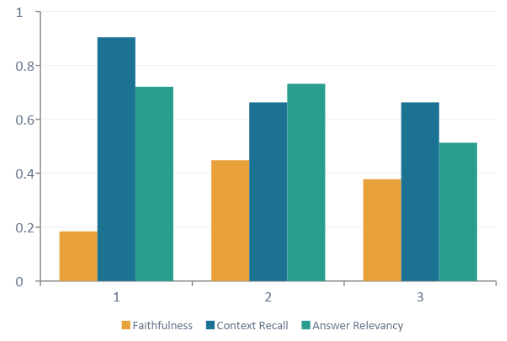
\includegraphics[width=0.85\textwidth]{figures/ragas_metrics.png}
    \caption{RAGAS metric comparison across the three pipeline variants.}
    \label{fig:ragas-metrics}
\end{figure}

\subsection{AI-Assisted Scoring and Human Review}

Aside from RAGAS, the V1 baseline was also evaluated using AI-assisted scoring and human review. The AI-assisted scoring used Qwen-2.5-3B as a local judge, while human review involved manually comparing the generated answers with the reference answers and source manuals. The results are shown in Table~\ref{tab:qwen-human}.

\begin{table}[t]
\centering
\caption{Comparison of AI-assisted scoring and human review for V1}
\label{tab:qwen-human}
\small
\setlength{\tabcolsep}{5pt}
\renewcommand{\arraystretch}{1.15}
\begin{tabularx}{0.85\textwidth}{@{}Y C{2.5cm} C{2.5cm}@{}}
\toprule
\textbf{Scoring Method} & \textbf{Strict Accuracy} & \textbf{Lenient Accuracy} \\
\midrule
Qwen-2.5-3B judge & 4\% & 26\% \\
Human review & 28\% & 50\% \\
\bottomrule
\end{tabularx}
\end{table}

The AI-assisted judge scored the baseline much lower than the human reviewers. Qwen-2.5-3B gave a strict accuracy of 4\%, while human review gave 28\%. For lenient accuracy, which gives partial credit to incomplete but relevant answers, Qwen gave 26\%, while human review gave 50\%.

This difference shows that the local LLM judge was stricter than human evaluation. The judge tended to penalize answers that missed exact details, even when the answer still contained relevant and useful information. Because of this, AI-assisted scoring was treated as a supporting evaluation method rather than the only basis for assessing system quality. Human review remained necessary to determine whether the answers were practically useful and aligned with the source manuals.

\subsection{Manual Classifier Results}

The manual classifier was evaluated using 5-fold cross-validation. It was trained to predict which manual a user query belongs to, allowing the system to automatically route questions before retrieval. The results are shown in Table~\ref{tab:classifier-results}.

\begin{table}[t]
\centering
\caption{Manual classifier validation accuracy}
\label{tab:classifier-results}
\small
\setlength{\tabcolsep}{6pt}
\renewcommand{\arraystretch}{1.15}
\begin{tabular}{@{}C{3cm} C{4cm}@{}}
\toprule
\textbf{Fold} & \textbf{Validation Accuracy} \\
\midrule
1 & 1.000 \\
2 & 1.000 \\
3 & 1.000 \\
4 & 0.950 \\
5 & 0.950 \\
\midrule
Mean & 0.980 $\pm$ 0.024 \\
\bottomrule
\end{tabular}
\end{table}

The classifier achieved a mean validation accuracy of 0.980 with a standard deviation of 0.024. This shows that the classifier was effective at identifying the correct manual within the prepared dataset. Its integration into the \texttt{/ask\_auto} endpoint improves usability because users do not need to manually select the correct product manual before asking a question.

However, this result should be interpreted with caution. The training data was expanded through deterministic paraphrasing, and cross-validation was performed over the augmented examples. This means that paraphrases of the same original question may appear in both training and validation folds. As a result, the reported accuracy is likely an upper-bound estimate. A stricter evaluation should group paraphrases of the same original question into the same fold.
